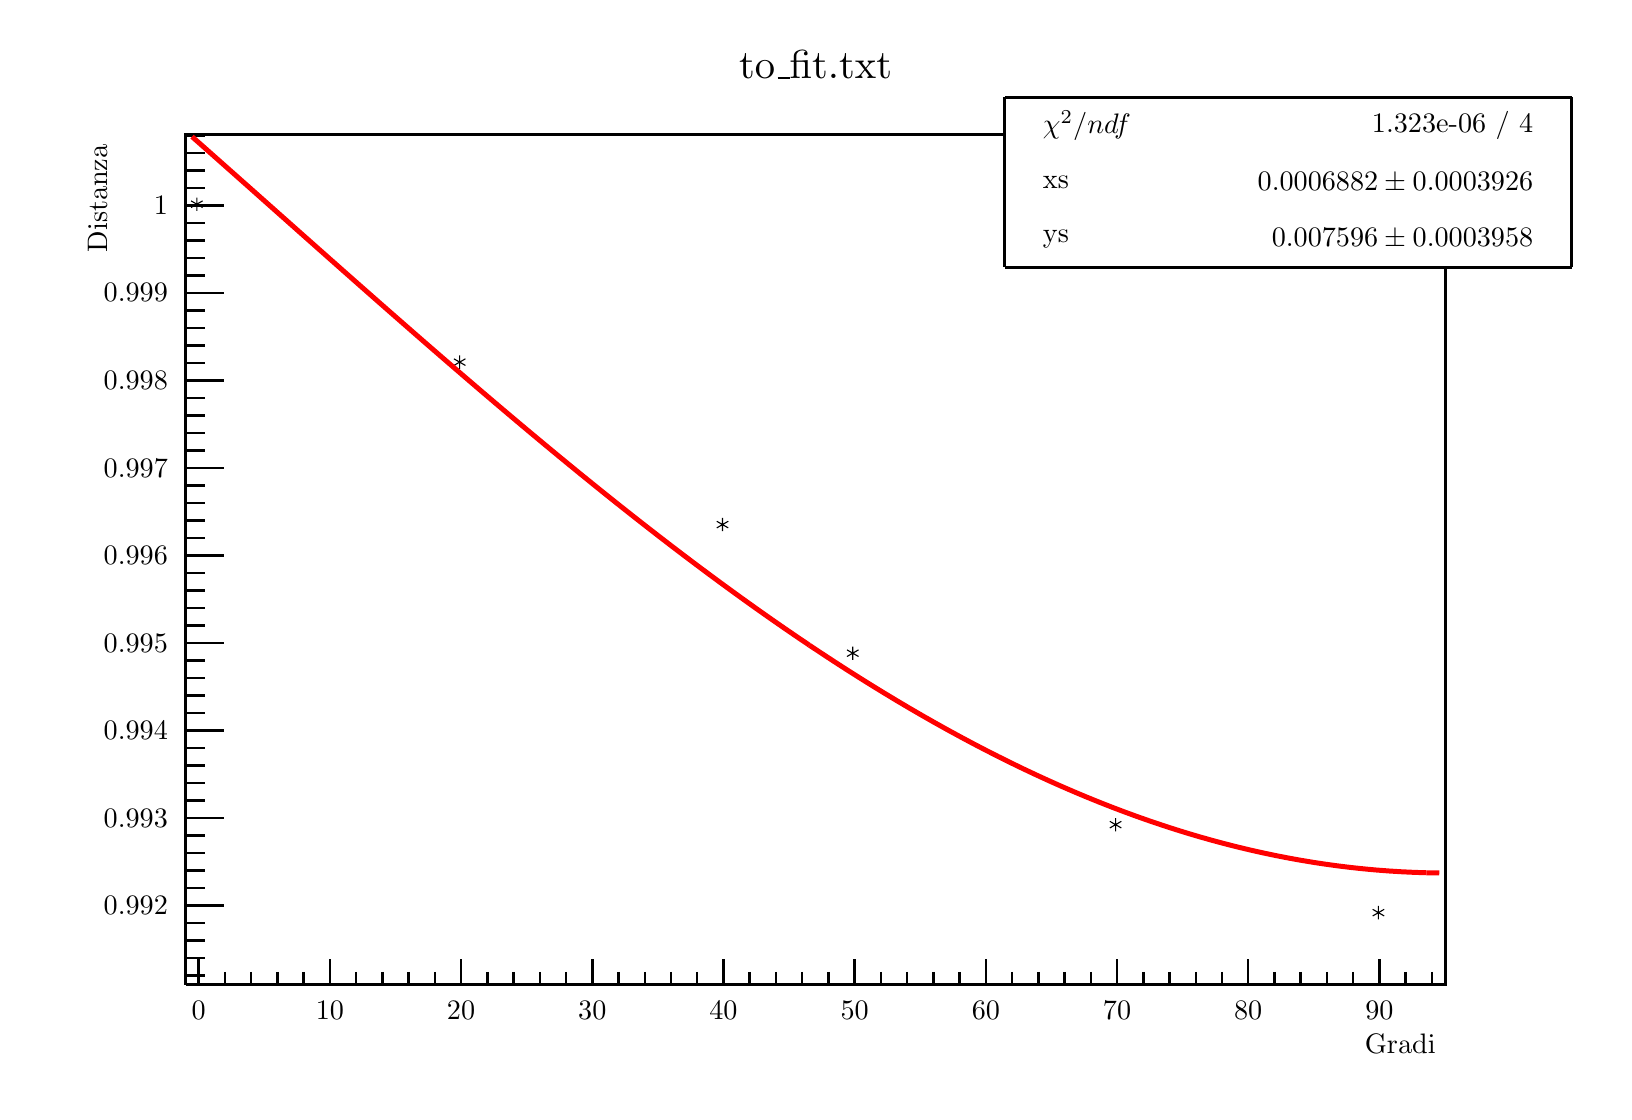
\begin{tikzpicture}
\pgfdeclareplotmark{cross} {
\pgfpathmoveto{\pgfpoint{-0.3\pgfplotmarksize}{\pgfplotmarksize}}
\pgfpathlineto{\pgfpoint{+0.3\pgfplotmarksize}{\pgfplotmarksize}}
\pgfpathlineto{\pgfpoint{+0.3\pgfplotmarksize}{0.3\pgfplotmarksize}}
\pgfpathlineto{\pgfpoint{+1\pgfplotmarksize}{0.3\pgfplotmarksize}}
\pgfpathlineto{\pgfpoint{+1\pgfplotmarksize}{-0.3\pgfplotmarksize}}
\pgfpathlineto{\pgfpoint{+0.3\pgfplotmarksize}{-0.3\pgfplotmarksize}}
\pgfpathlineto{\pgfpoint{+0.3\pgfplotmarksize}{-1.\pgfplotmarksize}}
\pgfpathlineto{\pgfpoint{-0.3\pgfplotmarksize}{-1.\pgfplotmarksize}}
\pgfpathlineto{\pgfpoint{-0.3\pgfplotmarksize}{-0.3\pgfplotmarksize}}
\pgfpathlineto{\pgfpoint{-1.\pgfplotmarksize}{-0.3\pgfplotmarksize}}
\pgfpathlineto{\pgfpoint{-1.\pgfplotmarksize}{0.3\pgfplotmarksize}}
\pgfpathlineto{\pgfpoint{-0.3\pgfplotmarksize}{0.3\pgfplotmarksize}}
\pgfpathclose
\pgfusepathqstroke
}
\pgfdeclareplotmark{cross*} {
\pgfpathmoveto{\pgfpoint{-0.3\pgfplotmarksize}{\pgfplotmarksize}}
\pgfpathlineto{\pgfpoint{+0.3\pgfplotmarksize}{\pgfplotmarksize}}
\pgfpathlineto{\pgfpoint{+0.3\pgfplotmarksize}{0.3\pgfplotmarksize}}
\pgfpathlineto{\pgfpoint{+1\pgfplotmarksize}{0.3\pgfplotmarksize}}
\pgfpathlineto{\pgfpoint{+1\pgfplotmarksize}{-0.3\pgfplotmarksize}}
\pgfpathlineto{\pgfpoint{+0.3\pgfplotmarksize}{-0.3\pgfplotmarksize}}
\pgfpathlineto{\pgfpoint{+0.3\pgfplotmarksize}{-1.\pgfplotmarksize}}
\pgfpathlineto{\pgfpoint{-0.3\pgfplotmarksize}{-1.\pgfplotmarksize}}
\pgfpathlineto{\pgfpoint{-0.3\pgfplotmarksize}{-0.3\pgfplotmarksize}}
\pgfpathlineto{\pgfpoint{-1.\pgfplotmarksize}{-0.3\pgfplotmarksize}}
\pgfpathlineto{\pgfpoint{-1.\pgfplotmarksize}{0.3\pgfplotmarksize}}
\pgfpathlineto{\pgfpoint{-0.3\pgfplotmarksize}{0.3\pgfplotmarksize}}
\pgfpathclose
\pgfusepathqfillstroke
}
\pgfdeclareplotmark{newstar} {
\pgfpathmoveto{\pgfqpoint{0pt}{\pgfplotmarksize}}
\pgfpathlineto{\pgfqpointpolar{44}{0.5\pgfplotmarksize}}
\pgfpathlineto{\pgfqpointpolar{18}{\pgfplotmarksize}}
\pgfpathlineto{\pgfqpointpolar{-20}{0.5\pgfplotmarksize}}
\pgfpathlineto{\pgfqpointpolar{-54}{\pgfplotmarksize}}
\pgfpathlineto{\pgfqpointpolar{-90}{0.5\pgfplotmarksize}}
\pgfpathlineto{\pgfqpointpolar{234}{\pgfplotmarksize}}
\pgfpathlineto{\pgfqpointpolar{198}{0.5\pgfplotmarksize}}
\pgfpathlineto{\pgfqpointpolar{162}{\pgfplotmarksize}}
\pgfpathlineto{\pgfqpointpolar{134}{0.5\pgfplotmarksize}}
\pgfpathclose
\pgfusepathqstroke
}
\pgfdeclareplotmark{newstar*} {
\pgfpathmoveto{\pgfqpoint{0pt}{\pgfplotmarksize}}
\pgfpathlineto{\pgfqpointpolar{44}{0.5\pgfplotmarksize}}
\pgfpathlineto{\pgfqpointpolar{18}{\pgfplotmarksize}}
\pgfpathlineto{\pgfqpointpolar{-20}{0.5\pgfplotmarksize}}
\pgfpathlineto{\pgfqpointpolar{-54}{\pgfplotmarksize}}
\pgfpathlineto{\pgfqpointpolar{-90}{0.5\pgfplotmarksize}}
\pgfpathlineto{\pgfqpointpolar{234}{\pgfplotmarksize}}
\pgfpathlineto{\pgfqpointpolar{198}{0.5\pgfplotmarksize}}
\pgfpathlineto{\pgfqpointpolar{162}{\pgfplotmarksize}}
\pgfpathlineto{\pgfqpointpolar{134}{0.5\pgfplotmarksize}}
\pgfpathclose
\pgfusepathqfillstroke
}
\definecolor{c}{rgb}{1,1,1};
\draw [color=c, fill=c] (0,0) rectangle (20,13.4957);
\draw [color=c, fill=c] (2,1.34957) rectangle (18,12.1461);
\definecolor{c}{rgb}{0,0,0};
\draw [c,line width=0.9] (2,1.34957) -- (2,12.1461) -- (18,12.1461) -- (18,1.34957) -- (2,1.34957);
\definecolor{c}{rgb}{1,1,1};
\draw [color=c, fill=c] (2,1.34957) rectangle (18,12.1461);
\definecolor{c}{rgb}{0,0,0};
\draw [c,line width=0.9] (2,1.34957) -- (2,12.1461) -- (18,12.1461) -- (18,1.34957) -- (2,1.34957);
\draw [c,line width=0.9] (2,1.34957) -- (18,1.34957);
\draw [anchor= east] (18,0.593811) node[scale=1.01821, color=c, rotate=0]{Gradi};
\draw [c,line width=0.9] (2.16495,1.67347) -- (2.16495,1.34957);
\draw [c,line width=0.9] (2.49818,1.51152) -- (2.49818,1.34957);
\draw [c,line width=0.9] (2.83141,1.51152) -- (2.83141,1.34957);
\draw [c,line width=0.9] (3.16464,1.51152) -- (3.16464,1.34957);
\draw [c,line width=0.9] (3.49787,1.51152) -- (3.49787,1.34957);
\draw [c,line width=0.9] (3.83109,1.67347) -- (3.83109,1.34957);
\draw [c,line width=0.9] (4.16432,1.51152) -- (4.16432,1.34957);
\draw [c,line width=0.9] (4.49755,1.51152) -- (4.49755,1.34957);
\draw [c,line width=0.9] (4.83078,1.51152) -- (4.83078,1.34957);
\draw [c,line width=0.9] (5.16401,1.51152) -- (5.16401,1.34957);
\draw [c,line width=0.9] (5.49724,1.67347) -- (5.49724,1.34957);
\draw [c,line width=0.9] (5.83047,1.51152) -- (5.83047,1.34957);
\draw [c,line width=0.9] (6.1637,1.51152) -- (6.1637,1.34957);
\draw [c,line width=0.9] (6.49693,1.51152) -- (6.49693,1.34957);
\draw [c,line width=0.9] (6.83016,1.51152) -- (6.83016,1.34957);
\draw [c,line width=0.9] (7.16339,1.67347) -- (7.16339,1.34957);
\draw [c,line width=0.9] (7.49662,1.51152) -- (7.49662,1.34957);
\draw [c,line width=0.9] (7.82984,1.51152) -- (7.82984,1.34957);
\draw [c,line width=0.9] (8.16307,1.51152) -- (8.16307,1.34957);
\draw [c,line width=0.9] (8.4963,1.51152) -- (8.4963,1.34957);
\draw [c,line width=0.9] (8.82953,1.67347) -- (8.82953,1.34957);
\draw [c,line width=0.9] (9.16276,1.51152) -- (9.16276,1.34957);
\draw [c,line width=0.9] (9.49599,1.51152) -- (9.49599,1.34957);
\draw [c,line width=0.9] (9.82922,1.51152) -- (9.82922,1.34957);
\draw [c,line width=0.9] (10.1624,1.51152) -- (10.1624,1.34957);
\draw [c,line width=0.9] (10.4957,1.67347) -- (10.4957,1.34957);
\draw [c,line width=0.9] (10.8289,1.51152) -- (10.8289,1.34957);
\draw [c,line width=0.9] (11.1621,1.51152) -- (11.1621,1.34957);
\draw [c,line width=0.9] (11.4954,1.51152) -- (11.4954,1.34957);
\draw [c,line width=0.9] (11.8286,1.51152) -- (11.8286,1.34957);
\draw [c,line width=0.9] (12.1618,1.67347) -- (12.1618,1.34957);
\draw [c,line width=0.9] (12.4951,1.51152) -- (12.4951,1.34957);
\draw [c,line width=0.9] (12.8283,1.51152) -- (12.8283,1.34957);
\draw [c,line width=0.9] (13.1615,1.51152) -- (13.1615,1.34957);
\draw [c,line width=0.9] (13.4947,1.51152) -- (13.4947,1.34957);
\draw [c,line width=0.9] (13.828,1.67347) -- (13.828,1.34957);
\draw [c,line width=0.9] (14.1612,1.51152) -- (14.1612,1.34957);
\draw [c,line width=0.9] (14.4944,1.51152) -- (14.4944,1.34957);
\draw [c,line width=0.9] (14.8277,1.51152) -- (14.8277,1.34957);
\draw [c,line width=0.9] (15.1609,1.51152) -- (15.1609,1.34957);
\draw [c,line width=0.9] (15.4941,1.67347) -- (15.4941,1.34957);
\draw [c,line width=0.9] (15.8273,1.51152) -- (15.8273,1.34957);
\draw [c,line width=0.9] (16.1606,1.51152) -- (16.1606,1.34957);
\draw [c,line width=0.9] (16.4938,1.51152) -- (16.4938,1.34957);
\draw [c,line width=0.9] (16.827,1.51152) -- (16.827,1.34957);
\draw [c,line width=0.9] (17.1603,1.67347) -- (17.1603,1.34957);
\draw [c,line width=0.9] (2.16495,1.67347) -- (2.16495,1.34957);
\draw [c,line width=0.9] (17.1603,1.67347) -- (17.1603,1.34957);
\draw [c,line width=0.9] (17.4935,1.51152) -- (17.4935,1.34957);
\draw [c,line width=0.9] (17.8267,1.51152) -- (17.8267,1.34957);
\draw [anchor=base] (2.16495,0.904212) node[scale=1.01821, color=c, rotate=0]{0};
\draw [anchor=base] (3.83109,0.904212) node[scale=1.01821, color=c, rotate=0]{10};
\draw [anchor=base] (5.49724,0.904212) node[scale=1.01821, color=c, rotate=0]{20};
\draw [anchor=base] (7.16339,0.904212) node[scale=1.01821, color=c, rotate=0]{30};
\draw [anchor=base] (8.82953,0.904212) node[scale=1.01821, color=c, rotate=0]{40};
\draw [anchor=base] (10.4957,0.904212) node[scale=1.01821, color=c, rotate=0]{50};
\draw [anchor=base] (12.1618,0.904212) node[scale=1.01821, color=c, rotate=0]{60};
\draw [anchor=base] (13.828,0.904212) node[scale=1.01821, color=c, rotate=0]{70};
\draw [anchor=base] (15.4941,0.904212) node[scale=1.01821, color=c, rotate=0]{80};
\draw [anchor=base] (17.1603,0.904212) node[scale=1.01821, color=c, rotate=0]{90};
\draw [c,line width=0.9] (2,1.34957) -- (2,12.1461);
\draw [anchor= east] (0.88,12.1461) node[scale=1.01821, color=c, rotate=90]{Distanza};
\draw [c,line width=0.9] (2.48,2.3521) -- (2,2.3521);
\draw [c,line width=0.9] (2.24,2.57446) -- (2,2.57446);
\draw [c,line width=0.9] (2.24,2.79682) -- (2,2.79682);
\draw [c,line width=0.9] (2.24,3.01918) -- (2,3.01918);
\draw [c,line width=0.9] (2.24,3.24153) -- (2,3.24153);
\draw [c,line width=0.9] (2.48,3.46389) -- (2,3.46389);
\draw [c,line width=0.9] (2.24,3.68625) -- (2,3.68625);
\draw [c,line width=0.9] (2.24,3.90861) -- (2,3.90861);
\draw [c,line width=0.9] (2.24,4.13097) -- (2,4.13097);
\draw [c,line width=0.9] (2.24,4.35332) -- (2,4.35332);
\draw [c,line width=0.9] (2.48,4.57568) -- (2,4.57568);
\draw [c,line width=0.9] (2.24,4.79804) -- (2,4.79804);
\draw [c,line width=0.9] (2.24,5.0204) -- (2,5.0204);
\draw [c,line width=0.9] (2.24,5.24276) -- (2,5.24276);
\draw [c,line width=0.9] (2.24,5.46511) -- (2,5.46511);
\draw [c,line width=0.9] (2.48,5.68747) -- (2,5.68747);
\draw [c,line width=0.9] (2.24,5.90983) -- (2,5.90983);
\draw [c,line width=0.9] (2.24,6.13219) -- (2,6.13219);
\draw [c,line width=0.9] (2.24,6.35454) -- (2,6.35454);
\draw [c,line width=0.9] (2.24,6.5769) -- (2,6.5769);
\draw [c,line width=0.9] (2.48,6.79926) -- (2,6.79926);
\draw [c,line width=0.9] (2.24,7.02162) -- (2,7.02162);
\draw [c,line width=0.9] (2.24,7.24398) -- (2,7.24398);
\draw [c,line width=0.9] (2.24,7.46633) -- (2,7.46633);
\draw [c,line width=0.9] (2.24,7.68869) -- (2,7.68869);
\draw [c,line width=0.9] (2.48,7.91105) -- (2,7.91105);
\draw [c,line width=0.9] (2.24,8.13341) -- (2,8.13341);
\draw [c,line width=0.9] (2.24,8.35577) -- (2,8.35577);
\draw [c,line width=0.9] (2.24,8.57812) -- (2,8.57812);
\draw [c,line width=0.9] (2.24,8.80048) -- (2,8.80048);
\draw [c,line width=0.9] (2.48,9.02284) -- (2,9.02284);
\draw [c,line width=0.9] (2.24,9.2452) -- (2,9.2452);
\draw [c,line width=0.9] (2.24,9.46756) -- (2,9.46756);
\draw [c,line width=0.9] (2.24,9.68991) -- (2,9.68991);
\draw [c,line width=0.9] (2.24,9.91227) -- (2,9.91227);
\draw [c,line width=0.9] (2.48,10.1346) -- (2,10.1346);
\draw [c,line width=0.9] (2.24,10.357) -- (2,10.357);
\draw [c,line width=0.9] (2.24,10.5793) -- (2,10.5793);
\draw [c,line width=0.9] (2.24,10.8017) -- (2,10.8017);
\draw [c,line width=0.9] (2.24,11.0241) -- (2,11.0241);
\draw [c,line width=0.9] (2.48,11.2464) -- (2,11.2464);
\draw [c,line width=0.9] (2.48,2.3521) -- (2,2.3521);
\draw [c,line width=0.9] (2.24,2.12975) -- (2,2.12975);
\draw [c,line width=0.9] (2.24,1.90739) -- (2,1.90739);
\draw [c,line width=0.9] (2.24,1.68503) -- (2,1.68503);
\draw [c,line width=0.9] (2.24,1.46267) -- (2,1.46267);
\draw [c,line width=0.9] (2.48,11.2464) -- (2,11.2464);
\draw [c,line width=0.9] (2.24,11.4688) -- (2,11.4688);
\draw [c,line width=0.9] (2.24,11.6911) -- (2,11.6911);
\draw [c,line width=0.9] (2.24,11.9135) -- (2,11.9135);
\draw [c,line width=0.9] (2.24,12.1358) -- (2,12.1358);
\draw [anchor= east] (1.9,2.3521) node[scale=1.01821, color=c, rotate=0]{0.992};
\draw [anchor= east] (1.9,3.46389) node[scale=1.01821, color=c, rotate=0]{0.993};
\draw [anchor= east] (1.9,4.57568) node[scale=1.01821, color=c, rotate=0]{0.994};
\draw [anchor= east] (1.9,5.68747) node[scale=1.01821, color=c, rotate=0]{0.995};
\draw [anchor= east] (1.9,6.79926) node[scale=1.01821, color=c, rotate=0]{0.996};
\draw [anchor= east] (1.9,7.91105) node[scale=1.01821, color=c, rotate=0]{0.997};
\draw [anchor= east] (1.9,9.02284) node[scale=1.01821, color=c, rotate=0]{0.998};
\draw [anchor= east] (1.9,10.1346) node[scale=1.01821, color=c, rotate=0]{0.999};
\draw [anchor= east] (1.9,11.2464) node[scale=1.01821, color=c, rotate=0]{1};
\definecolor{c}{rgb}{1,1,1};
\draw [color=c, fill=c] (12.4,10.4592) rectangle (19.6,12.6185);
\definecolor{c}{rgb}{0,0,0};
\draw [c,line width=0.9] (12.4,10.4592) -- (18,10.4592);
\draw [c,line width=0.9] (12.4,12.1461) -- (12.4,10.4592);
\draw [anchor= west] (12.76,12.2586) node[scale=1.01821, color=c, rotate=0]{$\chi^{2} / ndf $};
\draw [anchor= east] (19.24,12.2586) node[scale=1.01821, color=c, rotate=0]{ 1.323e-06 / 4};
\draw [anchor= west] (12.76,11.5388) node[scale=1.01821, color=c, rotate=0]{xs       };
\draw [anchor= east] (19.24,11.5388) node[scale=1.01821, color=c, rotate=0]{$ 0.0006882 \pm 0.0003926$};
\draw [anchor= west] (12.76,10.8191) node[scale=1.01821, color=c, rotate=0]{ys       };
\draw [anchor= east] (19.24,10.8191) node[scale=1.01821, color=c, rotate=0]{$ 0.007596 \pm 0.0003958$};
\foreach \P in {(2.14132,11.2607), (5.47928,9.25501), (8.81724,7.19198), (10.4714,5.55874), (13.8094,3.38109), (17.1474,2.26361)}{\draw[mark options={color=c,fill=c},mark size=2.402402pt,mark=asterisk] plot coordinates {\P};}
\definecolor{c}{rgb}{1,0,0};
\draw [c,line width=1.8] (2.08,12.1186) -- (2.24,11.9772) -- (2.4,11.8356) -- (2.56,11.6937) -- (2.72,11.5518) -- (2.88,11.4097) -- (3.04,11.2676) -- (3.2,11.1255) -- (3.36,10.9834) -- (3.52,10.8414) -- (3.68,10.6995) -- (3.84,10.5577) -- (4,10.4161)
 -- (4.16,10.2747) -- (4.32,10.1336) -- (4.48,9.99281) -- (4.64,9.85235) -- (4.8,9.71227) -- (4.96,9.57262) -- (5.12,9.43342) -- (5.28,9.29473) -- (5.44,9.15658) -- (5.6,9.01901) -- (5.76,8.88206) -- (5.92,8.74577) -- (6.08,8.61017) -- (6.24,8.4753)
 -- (6.4,8.34121) -- (6.56,8.20793) -- (6.72,8.07549) -- (6.88,7.94394) -- (7.04,7.81331) -- (7.2,7.68365) -- (7.36,7.55498) -- (7.52,7.42734) -- (7.68,7.30077) -- (7.84,7.17531) -- (8,7.05098) -- (8.16,6.92784) -- (8.32,6.8059) -- (8.48,6.68521) --
 (8.64,6.5658) -- (8.8,6.44771) -- (8.96,6.33096) -- (9.12,6.21559) -- (9.28,6.10164) -- (9.44,5.98913) -- (9.6,5.8781) -- (9.76,5.76858) -- (9.92,5.6606);
\draw [c,line width=1.8] (9.92,5.6606) -- (10.08,5.55419) -- (10.24,5.44939) -- (10.4,5.34621) -- (10.56,5.2447) -- (10.72,5.14488) -- (10.88,5.04678) -- (11.04,4.95042) -- (11.2,4.85584) -- (11.36,4.76306) -- (11.52,4.67211) -- (11.68,4.58302) --
 (11.84,4.4958) -- (12,4.41049) -- (12.16,4.3271) -- (12.32,4.24567) -- (12.48,4.16621) -- (12.64,4.08876) -- (12.8,4.01332) -- (12.96,3.93993) -- (13.12,3.8686) -- (13.28,3.79936) -- (13.44,3.73221) -- (13.6,3.6672) -- (13.76,3.60432) --
 (13.92,3.5436) -- (14.08,3.48506) -- (14.24,3.42872) -- (14.4,3.37458) -- (14.56,3.32267) -- (14.72,3.273) -- (14.88,3.22559) -- (15.04,3.18044) -- (15.2,3.13758) -- (15.36,3.09701) -- (15.52,3.05874) -- (15.68,3.0228) -- (15.84,2.98917) --
 (16,2.95789) -- (16.16,2.92895) -- (16.32,2.90236) -- (16.48,2.87814) -- (16.64,2.85628) -- (16.8,2.8368) -- (16.96,2.8197) -- (17.12,2.80498) -- (17.28,2.79265) -- (17.44,2.78272) -- (17.6,2.77518) -- (17.76,2.77003);
\draw [c,line width=1.8] (17.76,2.77003) -- (17.92,2.76729);
\definecolor{c}{rgb}{1,1,1};
\draw [color=c, fill=c] (12.4,10.4592) rectangle (19.6,12.6185);
\definecolor{c}{rgb}{0,0,0};
\draw [c,line width=0.9] (12.4,10.4592) -- (19.6,10.4592);
\draw [c,line width=0.9] (19.6,10.4592) -- (19.6,12.6185);
\draw [c,line width=0.9] (19.6,12.6185) -- (12.4,12.6185);
\draw [c,line width=0.9] (12.4,12.6185) -- (12.4,10.4592);
\draw [anchor= west] (12.76,12.2586) node[scale=1.01821, color=c, rotate=0]{$\chi^{2} / ndf $};
\draw [anchor= east] (19.24,12.2586) node[scale=1.01821, color=c, rotate=0]{ 1.323e-06 / 4};
\draw [anchor= west] (12.76,11.5388) node[scale=1.01821, color=c, rotate=0]{xs       };
\draw [anchor= east] (19.24,11.5388) node[scale=1.01821, color=c, rotate=0]{$ 0.0006882 \pm 0.0003926$};
\draw [anchor= west] (12.76,10.8191) node[scale=1.01821, color=c, rotate=0]{ys       };
\draw [anchor= east] (19.24,10.8191) node[scale=1.01821, color=c, rotate=0]{$ 0.007596 \pm 0.0003958$};
\draw (10,13.0328) node[scale=1.46368, color=c, rotate=0]{to\_fit.txt};
\end{tikzpicture}
